\documentclass[a4paper, 12pt]{article}
\usepackage[spanish]{babel}
\usepackage[utf8]{inputenc}
\usepackage{amsmath}
\usepackage{indentfirst}
\usepackage{graphicx}
\usepackage[colorinlistoftodos]{todonotes}
\usepackage{esint}
\usepackage{multicol}
\usepackage{listings}

\definecolor{codegreen}{rgb}{0,0.6,0}                                       
\definecolor{codegray}{rgb}{0.5,0.5,0.5}
\definecolor{codepurple}{rgb}{0.58,0,0.82}
\definecolor{backcolour}{rgb}{0.95,0.95,0.92}

 \lstdefinestyle{customc}{                                                       
    language=C,
    backgroundcolor=\color{backcolour},   
    commentstyle=\color{codegreen},
    keywordstyle=\color{magenta},
    numberstyle=\tiny\color{codegray},
    stringstyle=\color{codepurple},
    basicstyle=\ttfamily\footnotesize,
    breakatwhitespace=false,         
    breaklines=true,                 
    captionpos=b,                    
    keepspaces=true,                 
    numbers=left,                    
    numbersep=5pt,                  
    showspaces=false,                
    showstringspaces=false,                                                 
    showtabs=false,                  
    tabsize=2
}

\lstset{escapechar=@,style=customc}

 \lstset{literate=
  {á}{{\'a}}1 {é}{{\'e}}1 {í}{{\'i}}1 {ó}{{\'o}}1 {ú}{{\'u}}1
  {Á}{{\'A}}1 {É}{{\'E}}1 {Í}{{\'I}}1 {Ó}{{\'O}}1 {Ú}{{\'U}}1
  {à}{{\`a}}1 {è}{{\`e}}1 {ì}{{\`i}}1 {ò}{{\`o}}1 {ù}{{\`u}}1
  {À}{{\`A}}1 {È}{{\'E}}1 {Ì}{{\`I}}1 {Ò}{{\`O}}1 {Ù}{{\`U}}1
  {ä}{{\"a}}1 {ë}{{\"e}}1 {ï}{{\"i}}1 {ö}{{\"o}}1 {ü}{{\"u}}1
  {Ä}{{\"A}}1 {Ë}{{\"E}}1 {Ï}{{\"I}}1 {Ö}{{\"O}}1 {Ü}{{\"U}}1
  {â}{{\^a}}1 {ê}{{\^e}}1 {î}{{\^i}}1 {ô}{{\^o}}1 {û}{{\^u}}1
  {Â}{{\^A}}1 {Ê}{{\^E}}1 {Î}{{\^I}}1 {Ô}{{\^O}}1 {Û}{{\^U}}1
  {ã}{{\~a}}1 {ẽ}{{\~e}}1 {ĩ}{{\~i}}1 {õ}{{\~o}}1 {ũ}{{\~u}}1
  {Ã}{{\~A}}1 {Ẽ}{{\~E}}1 {Ĩ}{{\~I}}1 {Õ}{{\~O}}1 {Ũ}{{\~U}}1
  {œ}{{\oe}}1 {Œ}{{\OE}}1 {æ}{{\ae}}1 {Æ}{{\AE}}1 {ß}{{\ss}}1
  {ű}{{\H{u}}}1 {Ű}{{\H{U}}}1 {ő}{{\H{o}}}1 {Ő}{{\H{O}}}1
  {ç}{{\c c}}1 {Ç}{{\c C}}1 {ø}{{\o}}1 {å}{{\r a}}1 {Å}{{\r A}}1
  {€}{{\euro}}1 {£}{{\pounds}}1 {«}{{\guillemotleft}}1
  {»}{{\guillemotright}}1 {ñ}{{\~n}}1 {Ñ}{{\~N}}1 {¿}{{?`}}1 {¡}{{!`}}1  {°}    {{$^\circ$}}1
}

\setlength{\marginparwidth}{2cm}
\begin{document}
\begin{titlepage}
	\begin{center}
		{\large{UNIVERSIDAD TECNOLÓGICA NACIONAL}}
	\end{center}
	\vspace{15pt}
	\begin{figure}[!ht]
		\centering
		\begin{center}
			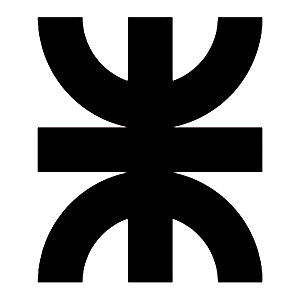
\includegraphics[width=5cm]{utn.png}
		\end{center}
	\end{figure}
	\vspace{5pt}
	\begin{center}
		{\large{FACULTAD REGIONAL PARANÁ}}
		\vspace{5pt}
		\begin{center}
			\vspace{15pt}
			\normalsize{CARRERA: Ingeniería Electrónica\\
						CÁTEDRA: Técnicas Digitales II\\}
			\vspace{50pt}
			\huge\bfseries{Trabajo Práctico N°7\\
				Medidor de frecuencia - simple\\}
\vspace{50pt}
		\end{center}
		
		\begin{flushleft}
			\begin{center}
				ALUMNOS:\\
				Battaglia Carlo\\
				Escobar Gabriel\\
			\end{center}
		\end{flushleft}
		
		\begin{center}
			\vspace{\fill}
			\normalsize{Paraná,}
			\today
		\end{center}
	\end{center}
\end{titlepage}

\newpage
\pagenumbering{arabic}
\numberwithin{equation}{section}

\section{Desarrollo}

\subsection{El circuito se basará en la placa Arduino UNO, si lo cree conveniente, puede agregar una etapa de “driver” entre el generador y la placa Arduino.}

\subsection{Se inyectará una señal cuadrada, desde un generador de funciones, a un pin convenientemente seleccionado, para la medición de la frecuencia.}

Para la generación de la señal cuadrada se utilizó un Arduino Mega2560 el cual ofrece una señal con una frecuencia de oscilación de $8[MHz]$, $1[MHz]$, $125[kHz]$, $31.25[kHz]$, $7.8125[kHz]$, cuyos valores se corresponden a la señal sin preescalado del $clock$, $clock/8$, $clock/64$, $clock/256$ y $clock/1024$ respectivamente.

\subsection{El funcionamiento general del circuito es:}

\subsubsection{Se inyectará una señal cuadrada y se deberá enviar el valor de la frecuencia en el monitor serie que trae el entorno de Microchip Studio.}

\subsubsection{El software del Arduino deberá hacer los ajustes de Hz, KHz, MHz, etc. cuando sea conveniente.}

\subsubsection{¿Qué sucede si le cambia el ciclo de trabajo a la señal del generador de funciones?}

Al cambiar el ciclo de trabajo a la señal del generador obtenemos el mismo funcionamiento debido a que la frecuencia de la señal no se ve afectada. Lo que varia es el instante donde la señal conmuta de un estado alto a uno bajo, pero como las interrupciones se producen únicamente en flancos ascendentes, el funcionamiento no se va a ver afectado debido a que el periodo de la señal continúa siendo el mismo.

\subsubsection{¿Qué sucede si le agrega un offset a la señal del generador de funciones?}

Al agregar un offset a la señal se corre el riesgo de que, en cierto momento, la señal deje de operar como una señal cuadrada debido al efecto Schmitt Trigger que poseen las entradas (de PWM) del Arduino UNO.

Este efecto determina dos umbrales diferentes para establecer que la señal se encuentra en un estado lógico ``HIGH'' (alto) o un estado lógico ``LOW'' (bajo), por lo que si el offset agregado es tal que alcance el umbral inferior, una vez que la señal este en alto, por más que conmute, no llegara a tomar un valor bajo nuevamente y será tomada como una señal que se encuentra constantemente en alto por lo tanto no existirá conmutación y no se producirán interrupciones debido a que no se lograran distinguir los flancos ascendentes.

\subsubsection{¿Qué sucede si ingresa una sinusoidal?}

Si ingresa una señal sinusoidal producirá un efecto similar al de la señal cuadrada debido a que una vez que se detecte que esta supere el umbral superior de la entrada del Arduino se tomará como una señal en alto y una vez que decaiga por debajo del umbral inferior se la tomará como una señal en bajo. La frecuencia de la señal no se verá afectada.

\subsubsection{¿Qué sucede si ingresa una triangular?}

Ídem inciso anterior.

\section{Código}

\small{\lstinputlisting[language=C]{medidor_freq/medidor_freq.ino}}
 
\end{document}
